\documentclass{article}
\usepackage[paperwidth=18.8cm,paperheight=10.0cm,margin=0cm]{geometry}
\usepackage{tikz}
\usepackage{amsmath,amssymb}
\usetikzlibrary{arrows.meta,calc,positioning}
\pagestyle{empty}
\setlength{\parindent}{0pt}

\begin{document}
\noindent
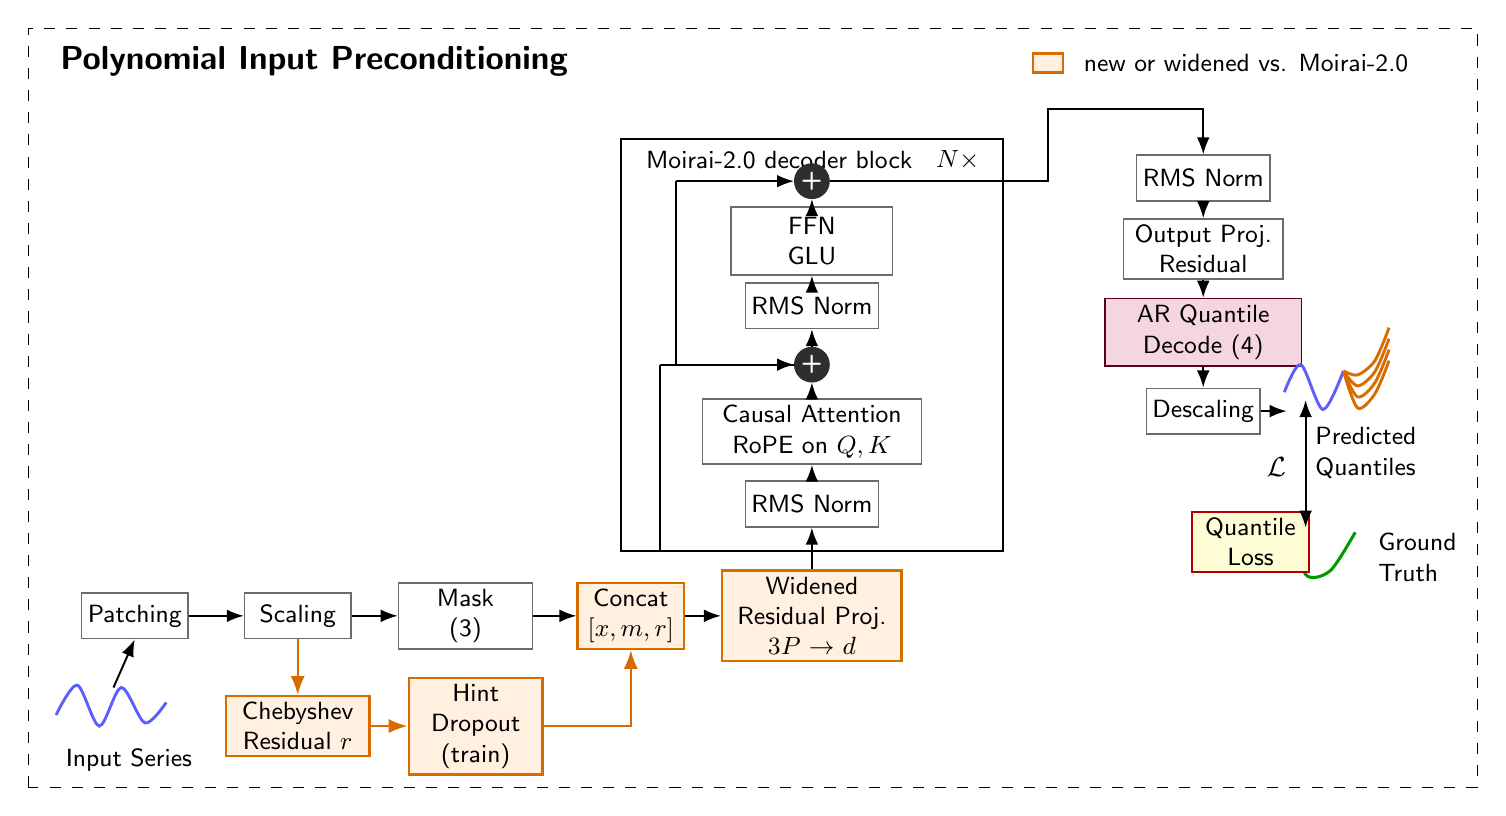
\begin{tikzpicture}[
    x=1cm,y=1cm,
    font=\sffamily,
    >=Latex,
    box/.style={
        draw=black!58,
        line width=0.55pt,
        fill=white,
        align=center,
        minimum height=0.58cm,
        inner sep=2.2pt,
        font=\sffamily\small
    },
    smallbox/.style={box, minimum width=1.35cm},
    medbox/.style={box, minimum width=1.70cm},
    widebox/.style={box, minimum width=2.25cm},
    changed/.style={
        box,
        draw=orange!85!black,
        fill=orange!12,
        line width=0.85pt
    },
    flow/.style={->, line width=0.70pt, draw=black},
    hintflow/.style={->, line width=0.85pt, draw=orange!85!black},
    wire/.style={line width=0.70pt, draw=black},
    sum/.style={
        circle,
        fill=black!82,
        draw=black!82,
        text=white,
        minimum size=0.44cm,
        inner sep=0pt,
        font=\sffamily\bfseries\small
    }
]

% -----------------------------------------------------------------------------
% Panel and legend
% -----------------------------------------------------------------------------
\draw[dashed, line width=0.55pt, dash pattern=on 4pt off 4pt]
    (0.20,0.18) rectangle (18.60,9.82);

\node[font=\sffamily\bfseries\large, anchor=west] at (0.48,9.40)
    {Polynomial Input Preconditioning};
\node[changed, minimum width=0.38cm, minimum height=0.24cm] at (13.15,9.38) {};
\node[font=\sffamily\small, anchor=west] at (13.48,9.38)
    {new or widened vs. Moirai-2.0};

% -----------------------------------------------------------------------------
% Input and modified input projection
% -----------------------------------------------------------------------------
\draw[blue!63, line width=1.05pt]
    plot[smooth] coordinates {(0.55,1.10) (0.82,1.48) (1.10,0.96)
        (1.38,1.45) (1.68,1.00) (1.95,1.26)};
\node[anchor=west, font=\sffamily\small] at (0.55,0.52) {Input Series};

\node[smallbox] (patch) at (1.55,2.36) {Patching};
\node[smallbox] (scale) at (3.62,2.36) {Scaling};
\node[medbox] (mask) at (5.75,2.36) {Mask\\(3)};
\node[changed, minimum width=1.35cm, text width=1.18cm] (cat) at (7.85,2.36)
    {Concat\\$[x,m,r]$};
\node[changed, minimum width=2.28cm, text width=2.08cm] (inproj) at (10.15,2.36)
    {Widened\\Residual Proj.\\$3P\!\to\! d$};

\node[changed, minimum width=1.82cm, text width=1.66cm] (resid) at (3.62,0.96)
    {Chebyshev\\Residual $r$};
\node[changed, minimum width=1.70cm, text width=1.52cm] (hdrop) at (5.88,0.96)
    {Hint Dropout\\(train)};

\draw[flow] (1.28,1.45) -- (patch.south);
\draw[flow] (patch.east) -- (scale.west);
\draw[flow] (scale.east) -- (mask.west);
\draw[flow] (mask.east) -- (cat.west);
\draw[flow] (cat.east) -- (inproj.west);

\draw[hintflow] (scale.south) -- (resid.north);
\draw[hintflow] (resid.east) -- (hdrop.west);
\draw[hintflow] (hdrop.east) -- (7.85,0.96) -- (cat.south);

% -----------------------------------------------------------------------------
% Unchanged transformer decoder block
% -----------------------------------------------------------------------------
\coordinate (Tsw) at (7.72,3.18);
\coordinate (Tne) at (12.58,8.42);
\draw[wire] (Tsw) rectangle (Tne);
\node[font=\sffamily\small, anchor=east] at (12.40,8.15) {$N{\times}$};
\node[font=\sffamily\small, anchor=west] at (7.92,8.15)
    {Moirai-2.0 decoder block};

\node[smallbox] (rms1) at (10.15,3.78) {RMS Norm};
\node[widebox, minimum width=2.78cm] (attn) at (10.15,4.70)
    {Causal Attention\\RoPE on $Q,K$};
\node[sum] (add1) at (10.15,5.55) {+};
\node[smallbox] (rms2) at (10.15,6.30) {RMS Norm};
\node[widebox, minimum width=2.05cm, minimum height=0.86cm] (ffn) at (10.15,7.12)
    {FFN\\GLU};
\node[sum] (add2) at (10.15,7.88) {+};

\coordinate (tin) at (10.15,3.18);
\draw[flow] (inproj.north) -- (tin) -- (rms1.south);
\draw[flow] (rms1.north) -- (attn.south);
\draw[flow] (attn.north) -- (add1.south);
\draw[flow] (add1.north) -- (rms2.south);
\draw[flow] (rms2.north) -- (ffn.south);
\draw[flow] (ffn.north) -- (add2.south);

\draw[wire] (tin) -- (8.22,3.18) -- (8.22,5.55);
\draw[flow] (8.22,5.55) -- (add1.west);
\draw[wire] (add1.west) -- (8.42,5.55) -- (8.42,7.88);
\draw[flow] (8.42,7.88) -- (add2.west);

% -----------------------------------------------------------------------------
% Unchanged output head and loss
% -----------------------------------------------------------------------------
\node[smallbox] (outrms) at (15.12,7.92) {RMS Norm};
\node[widebox, minimum width=2.02cm] (outproj) at (15.12,7.02)
    {Output Proj.\\Residual};
\node[
    box,
    draw=purple!45!black,
    fill=purple!16,
    minimum width=2.50cm,
    minimum height=0.86cm,
    text width=2.30cm
] (decode) at (15.12,5.96) {AR Quantile\\Decode (4)};
\node[smallbox] (descale) at (15.12,4.96) {Descaling};

\draw[flow] (add2.east) -- (13.15,7.88) -- (13.15,8.80) -- (15.12,8.80) -- (outrms.north);
\draw[flow] (outrms.south) -- (outproj.north);
\draw[flow] (outproj.south) -- (decode.north);
\draw[flow] (decode.south) -- (descale.north);

\draw[flow] (descale.east) -- (16.18,4.96);
\draw[blue!63, line width=1.05pt]
    plot[smooth] coordinates {(16.15,5.20) (16.36,5.55) (16.64,4.98) (16.90,5.47)};
\foreach \dy in {-0.18,-0.04,0.10,0.24} {
    \draw[orange!85!black, line width=1.05pt]
        plot[smooth] coordinates {(16.90,5.47) (17.08,5.18+\dy)
            (17.30,5.36+\dy) (17.48,5.78+\dy)};
}
\node[align=left, font=\sffamily\small, anchor=west] at (16.42,4.43)
    {Predicted\\Quantiles};

\draw[green!60!black, line width=1.10pt]
    plot[smooth] coordinates {(16.25,3.20) (16.45,2.86) (16.74,2.94) (17.05,3.42)};
\node[align=left, font=\sffamily\small, anchor=west] at (17.22,3.10)
    {Ground\\Truth};
\node[
    box,
    fill=yellow!16,
    draw=red!70!black,
    minimum width=1.48cm,
    text width=1.28cm
] (loss) at (15.72,3.30) {Quantile\\Loss};
\draw[<->, line width=0.70pt] (16.42,5.10) -- (16.42,3.48);
\node[font=\sffamily\normalsize] at (16.05,4.25) {$\mathcal{L}$};

\end{tikzpicture}
\end{document}
